\section{Proposed Approach}
\label{sec:approach}

\subsection{Multilingual CTC Model}
\begin{figure}[t]
    \centering
    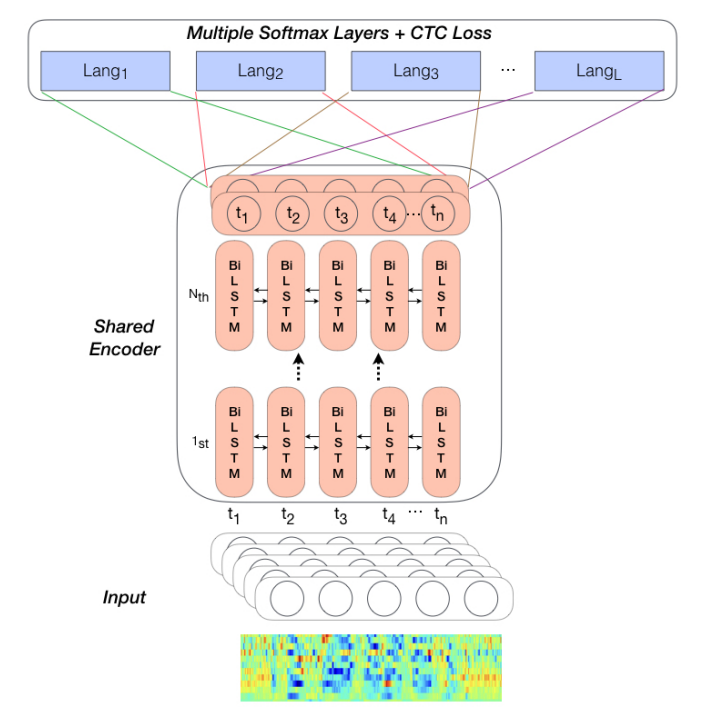
\includegraphics[width=\linewidth]{figs/model_arch.png}
    \caption{Multilingual CTC Model Architecture \textcolor{red}{WILL BE REPLACED}}
    \label{fig:model-arch}
    %\vspace{-10pt}
\end{figure}

We used the network architecture as illustrated in Fig. \ref{fig:model-arch}. Let $X = x_1, x_2, \cdots, x_T$ with length $T$ as input feature, $C = c_1, c_2, \cdots, c_L$ with length $L$ as target label. $X$ is encoded into sequence of hidden states $H = h_1, h_2, \cdots, h_L$ through the shared encoder, then fed into the fully connected layer of corresponding language with softmax activation to output the prediction sequence $\hat{C} = \hat{c_1}, \hat{c_2}, \cdots, \hat{c_L}$.
%\vspace{-2pt}

\textbf{CTC Loss}. CTC computes the posterior probability as below,

\begin{equation}
  P(C|X) = \sum_{\pi \in \mathcal{Z}(C)} P(\pi|X)
\end{equation}
where $\pi$ is the repeated character sequence  of $C$ with additional blank label, and $\mathcal{Z}(C)$ is the set of all possible sequences $\pi$ given sequence $C$. For each $\pi$, we can approximate the posterior probability as below,

\begin{equation}
  P(\pi|X) \approx \prod_{i=1}^{L} P(\hat{c_i}|X)
\end{equation}

The loss function of the model is thus defined as:

\begin{equation}
  L = - \log P(C|X)
\end{equation}

\subsection{Meta Learning for Low-Resource ASR}

%\begin{table*}[ht!]
\centering
\caption{Character (\% CER)  error rate w.r.t the pretraining languages set for all 4 target languages' FLP}
\label{tab:block-results}
\begin{tabular}{@{}ccccccccc@{}}
%\begin{tabular}{l|cc|cc|cc|cc}
\toprule
Model                                    & \multicolumn{2}{c}{Vietnamese}                         & \multicolumn{2}{c}{Swahili}                        & \multicolumn{2}{c}{Tamil}                        & \multicolumn{2}{c}{Kurmanji} \\

                                         & multi           & meta                                & multi           & meta                                & multi           & meta                                & multi           & meta           \\ \midrule
\multicolumn{1}{c|}{- (no-pretrain)}         & 100.0          & \multicolumn{1}{c|}{100.0}          & 100.0          & \multicolumn{1}{c|}{100.0}          & 100.0          & \multicolumn{1}{c|}{100.0}          & 100.0          & 100.0          \\

\multicolumn{1}{c|}{Bn Tl Zu}   & 53.2          & \multicolumn{1}{c|}{36.5}          & 52.8          & \multicolumn{1}{c|}{34.4}          & 47.8          & \multicolumn{1}{c|}{34.9}          & 55.9          & 41.1          \\
\multicolumn{1}{c|}{ Tr Lt Gn} & 50.6          & \multicolumn{1}{c|}{35.1}          & 49.0          & \multicolumn{1}{c|}{32.2}          & 46.6          & \multicolumn{1}{c|}{33.2}          & 53.4          & 39.6          \\
\multicolumn{1}{c|}{Bn Tl Zu Tr Lt Gn}           & 52.3          & \multicolumn{1}{c|}{36.6}          & 51.3          & \multicolumn{1}{c|}{33.0}          & 45.8          & \multicolumn{1}{c|}{33.9}          & 54.5          & 40.2          \\ \bottomrule
%\multicolumn{1}{c|}{MLing + SWBD \& FT}       & \textbf{48.2} & \multicolumn{1}{c|}{\textbf{33.5}} & \textbf{48.7} & \multicolumn{1}{c|}{\textbf{31.9}} & \textbf{44.3} & \multicolumn{1}{c|}{\textbf{31.9}} & \textbf{51.5} & \textbf{37.8} \\ \bottomrule
\end{tabular}
\end{table*}


%% ref: http://pgfplots.net/tikz/examples/bar-plot/
\begin{figure}[t]
\begin{minipage}[b]{1.0\linewidth}
    \raggedright
    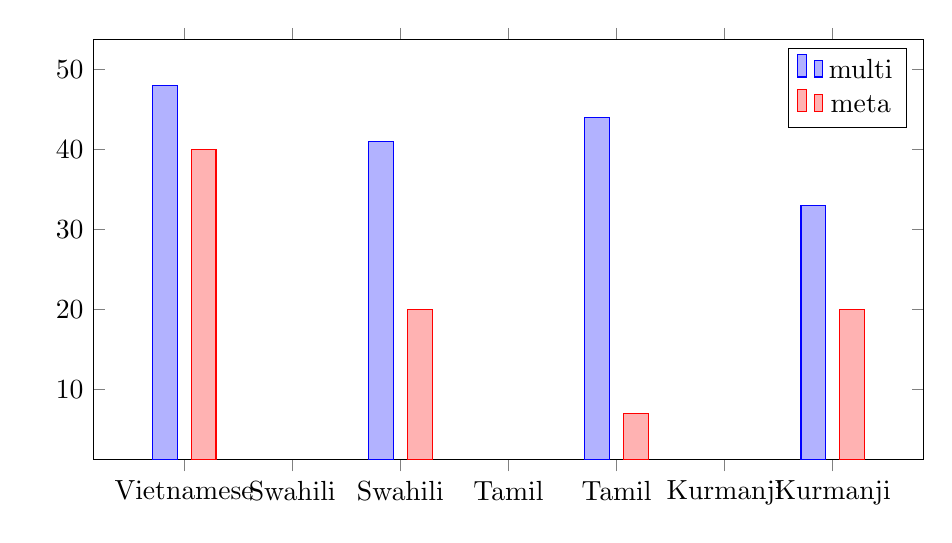
\begin{tikzpicture}
\begin{axis}[
	x tick label style={
		/pgf/number format/1000 sep=},
    ylabel= {\si{\percent}},
	enlargelimits=0.14,
	symbolic x coords={Vietnamese,Swahili,Tamil,Kurmanji},
	xticklabel style={align=center},
	ybar=5pt,
	height=.57\textwidth,
	width=\textwidth,
	bar width=9pt,
]

\addplot 
	coordinates {(Vietnamese,48) (Swahili,41)
		 (Tamil,44) (Kurmanji,33) };

\addplot 
	coordinates {(Vietnamese,40) (Swahili,20) 
		(Tamil,7) (Kurmanji,20) };

\legend{multi, meta}
\end{axis}
\end{tikzpicture}
\caption{CER relative improvement from LLP to FLP \textcolor{red}{Waiting for stat}}
    \label{fig:impact-on-size}
\end{minipage}

\end{figure}

%\begin{figure}[htpb]
    \centering
    \includegraphics[width=\linewidth]{figs/curve.pdf}
    \caption{The learning curves of BLEU scores on the validation task (Ro-En).}
    \label{fig:train curve}
    \vspace{-10pt}
\end{figure}



